\chapter{Sieci komputerowe}

Materiały teoretyczne zostały opracowane na podstawie \href{https://moodle.mimuw.edu.pl/course/view.php?id=1351}{slajdów Agaty Janowskiej}.

\section*{Podstawa programowa}
\begin{enumerate}
    \item \textbf{Warstwy sieci}.
    \item \textbf{Protokoły} TCP, UDP, IP, ICMP, Ethernet.
    \item \textbf{Adresy internetowe}, tablice tras, zasady trasowania, NAT.
    \item Systemy \textbf{nazw domenowych}.
    \item Sieciowy \textbf{interfejs gniazd}.
\end{enumerate}

% Jasiek
\section{Warstwy sieci}
Sieć możemy podzielić na warstwy, z których każda operuje na coraz niższym poziomie abstrakcji. Zalety takiego podziału to m.in.:
\begin{itemize}
    \item łatwiejsze definiowanie składników dużego systemu
    \item wyższa warstwa korzysta z usług oferowanych przez niższą warstwę
    \item modularność ułatwia zmiany
    \item w skład warstwy wchodzą protokoły wraz z urządzeniami i oprogramowaniem
    \item stos protokołów - kombinacja protokołów różnych warstw
\end{itemize}

\begin{figure}[H]
    \centering
    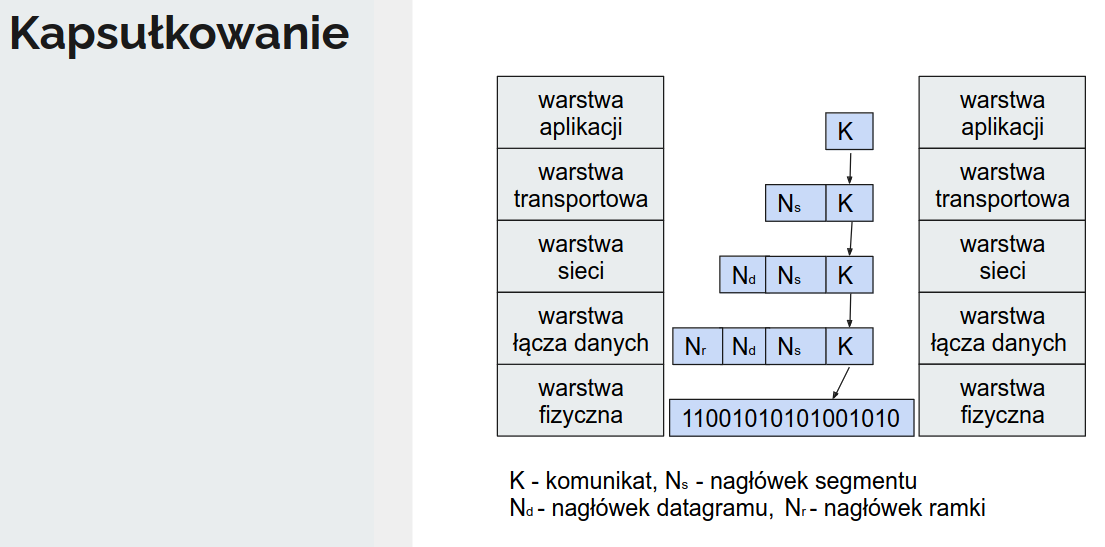
\includegraphics[scale=0.3]{rozdziały/images/SIK/encapsulation.png}
    \caption{Wizualizacja przekazywania komunikatów do kolejnych warstw}
\end{figure}


\subsection{Warstwa aplikacji}
Aplikacje sieciowe to programy uruchamiane na różnych systemach końcowych, komunikujące się ze sobą za pośrednictwem sieci np. przeglądarka internetowa z serwerem WWW. Wyróżniamy dwa główne podejścia:
\begin{enumerate}
    \item[1.] \textbf{Architektura klient-serwer}
        \begin{itemize}
            \item serwer obsługuje żądania klientów
            \item klienty nie komunikują się bezpośrednio ze sobą
            \item najczęściej serwer posiada ogólnie znany adres IP i jest cały czas dostępny
            \item przykłady: poczta elektroniczna, przeglądarki, zdalne logowanie
            \item zamiast pojedynczego serwera mogą być grupy serwerów, centra danych np. Amazon
        \end{itemize}
    \item[2.] \textbf{Architektura P2P (ang. Peer-to-Peer)}
        \begin{itemize}
            \item sieć równorzędna, bez pośrednictwa serwera
            \item aplikacje wykorzystują bezpośrednie połączenia między parami komunikujących się hostów nazywanych węzłami
            \item węzłami są systemy końcowe użytkowników
            \item sieci dystrybucji plików (np. BitTorrent), systemy wideokonferencji (np. Skype)
            \item samoskalowalne, tanie
            \item niski poziom bezpieczeństwa, niezawodności, wydajności
        \end{itemize}
\end{enumerate}

Protokół warstwy aplikacji określa w jaki sposób procesy wymieniają się komunikatami, czyli definiuje:
\begin{itemize}
    \item typy komunikatów
    \item składnię różnego typu komunikatów
    \item semantykę, czyli znaczenie poszczególnych pól komunikatu
    \item zasady mówiące kiedy i w jaki sposób proces wysyła komunikaty i na nie odpowiada
\end{itemize}

Główny protokół: \textbf{HTTP} stanowiący podstawowy składnik technologii WWW. W warstwie transportowej korzysta z protokołu TCP.


\subsection{Warstwa transportowa}
Odpowiada za przekazanie komunikatów między procesami tworzącymi aplikację w sposób \textbf{połączeniowy} (TCP) lub \textbf{bezpołączeniowy} (UDP). Warstwa transportowa po stronie nadawcy
dzieli komunikaty otrzymane od aplikacji na mniejsze fragmenty i dodaje do nich nagłówki warstwy transportowej tworząc \textbf{segmenty}. Następnie
\begin{itemize}
    \item segment przekazywany jest warstwie sieci;
    \item warstwa sieci kapsułkuje segment we własnym pakiecie (datagramie) i stara się go dostarczyć do odbiorcy;
    \item po stronie odbiorcy warstwa sieci wyodrębnia z datagramu segment i przekazuje go warstwie transportowej;
    \item warstwa transportowa przetwarza segment i przekazuje dane aplikacji odbiorczej.
\end{itemize}

Zadania warstwy transportowej:
\begin{itemize}
    \item multipleksowanie w warstwie transportowej – tworzenie segmentów i przekazanie ich warstwie sieci
    \item demultipleksowanie w warstwie transportowej – dostarczenie danych zawartych w segmentach do odpowiedniego procesu
    \item kontrola błędów (choć w UDP tylko trochę)
    \item zapewnienie niezawodnej usługi transferu danych (tylko TCP)
    \item kontrola przepływu (tylko TCP)
    \item kontrola przeciążenia (tylko TCP)
\end{itemize}


\subsection{Warstwa sieci}
Główne cechy:
\begin{itemize}
    \item wykorzystanie protokołu IP (Internet Protocol)
    \item cel: niegwarantowany (ang. best-effort), bezpołączeniowy transfer danych
    \begin{itemize}
        \item adresacja (IPv4, IPv6)
        \item trasowanie
    \end{itemize}
    \item protokoły DHCP, ICMP
    \item NAT
    \item przekazywanie \textbf{datagramów} między dowolnymi hostami
\end{itemize}


\subsection{Warstwa łącza danych}
Główne cechy:
\begin{itemize}
    \item przekazywanie danych pojedynczym łączem między \textbf{sąsiednimi} węzłami
    \begin{itemize}
        \item \textbf{ramkowanie}
        \item dostęp do łącza
        \item detekcja i usuwanie błędów (np. suma kontrolna, CRC)
    \end{itemize}
    \item implementacja może być
    \begin{itemize}
        \item sprzętowa na karcie sieciowej
        \item programowa
    \end{itemize}
\end{itemize}

Typy kanałów:
\begin{itemize}
    \item kanały rozgłaszania
    \begin{itemize}
        \item wiele hostów podłączonych do tego samego kanału komunikacyjnego
        \item np. bezprzewodowe sieci lokalne, satelitarne, hybrydowe używające światłowodu i kabla koncentrycznego
        \item konieczny protokół wielodostępu do nośnika
    \end{itemize}
    \item łącza punkt-punkt
    \begin{itemize}
        \item na przykład między dwoma routerami powiązanymi łączem czy komputerem i przełącznikiem (ang. switch)
    \end{itemize}
\end{itemize}

Adresy MAC:
\begin{itemize}
    \item każdy interfejs posiada adres MAC (ang. Media Access Control) (uwaga: przełączniki nie mają adresów MAC)
    \item 48-bitowy, wyrażany w notacji szesnastkowej z dwukropkami lub myślnikami
    \item adresy MAC zaprojektowano jako stałe, ale obecnie można je zmienić programowo
    \item unikalny, organizacja IEEE zarządza przestrzenią adresów, przydziela producentom kart sieciowych bloki liczące $2^{24}$ adresów
    \item płaska struktura, nie zmienia się wraz ze zmianą lokalizacji
\end{itemize}

Przesyłanie ramek:
\begin{itemize}
    \item nadawca umieszcza w ramce adres odbiorcy i przesyła ją do łącza
    \item kiedy karta sieciowa innego hosta otrzymuje ramkę, która nie jest do niej adresowana, odrzuca ją
    \item jeśli docelowy adres MAC pasuje do adresu MAC karty sieciowej, z ramki wyodrębniany jest datagram, który jest przekazywany w górę stosu protokołów
    \item karta sieciowa wpływa na pracę hosta, tylko jeżeli otrzyma adresowaną do niego ramkę
    \item adres rozgłoszeniowy FF:FF:FF:FF:FF:FF "pasuje" do każdego adresu MAC
    \item nadawca poznaje adres MAC odbiorcy poprzez \textbf{protokół ARP}
\end{itemize}


\subsection{Warstwa fizyczna}
Fizyczne nośniki:
\begin{itemize}
    \item skrętka nieekranowa
    \begin{itemize}
        \item najtańszy i najbardziej popularny nośnik
        \item dwa izolowane przewody miedziane, skręcone, aby zlikwidować zakłócenia elektryczne
    \end{itemize}
    \item światłowód
    \begin{itemize}
        \item cienki, elastyczny nośnik przenoszący impulsy świetlne
        \item stosowany tam, gdzie nie można zastosować skrętki (np. większe odległości)
        \item odporny na zakłócenie elektromagnetyczne, znikome tłumienie sygnału
    \end{itemize}
\end{itemize}

Ethernet - najpopularniejsza technologia sieci "przewodowej" opisana w szczegółach niżej.

\begin{figure}[H]
    \centering
    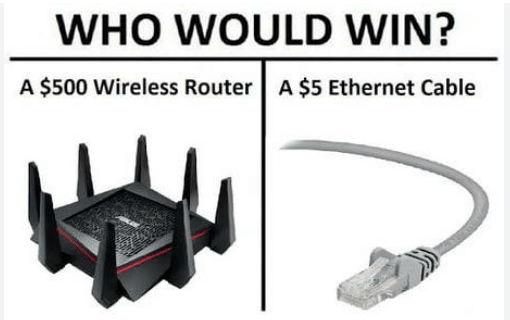
\includegraphics[scale=0.5]{rozdziały/images/SIK/ethernet_cable.png}
    \caption{Graficzne przedstawienie genetycznej dominacji potężnego kabla Ethernet}
\end{figure}


% Kasia, Jasiek
\section{Protokoły TCP, UDP, IP, ICMP, Ethernet}

\subsection{UDP}
Protokołowi temu przyświeca motto: "być może nie wszystkie dane przeżyją, ale jest to poświęcenie, na które jestem gotów". Główne cechy:
\begin{itemize}
    \item oferuje minimalną funkcjonalność jaką musi zapewnić warstwa transportowa: multipleksowanie i demultipleksowanie
    \item nie zapewnia niezawodności poza podstawową kontrolą błędów
    \item jest bezpołączeniowy
    \begin{itemize}
        \item odbiera komunikat od procesu aplikacji
        \item dołącza numery portów źródłowego i docelowego
        \item dodaje dwa niewielkie pola i przekazuje warstwie sieci
        \item po stronie odbiorcy wykorzystuje numer portu, aby odnaleźć odpowiedni proces aplikacji
    \end{itemize}
\end{itemize}

\begin{figure}[H]
    \centering
    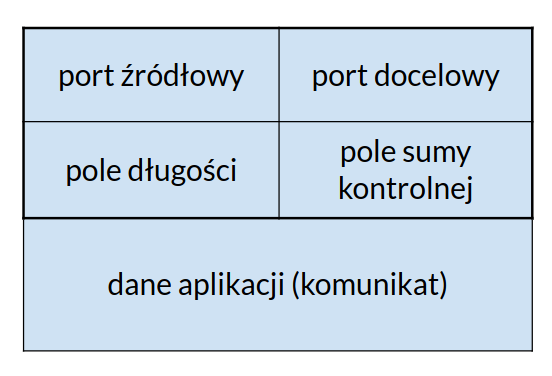
\includegraphics[scale=0.3]{rozdziały/images/SIK/udp_structure.png}
    \caption{Protokół UDP, struktura segmentu}
\end{figure}


\subsection{TCP}
Zadaniem TCP jest zapewnienie \textbf{niezawodnego} transferu danych. W tym celu wykorzystuje on poniższe tricki:
\begin{itemize}
    \item suma kontrolna: wykrywanie uszkodzeń pakietu
    \item mechanizm potwierdzeń: pozytywne (wszystko doszło, jest okej) i negatywne (coś poszło źle)
    \item jeśli dane uszkodzone -- retransmisja
    \item jeśli potwierdzenie uszkodzone -- retransmisja
    \item właściwa kolejność danych -- numery sekwencyjne
    \item wykrywanie \textbf{utraty} pakietu -- potrzebne zegary, oczekiwanie na potwierdzenie przez określony czas (czyli większy niż RTT: ang. Round-Trip Time)
    \item wykrycie utraty pakietu oczywiście powoduje retransmisję
    \item aby nadawca nie musiał czekać po wysłaniu każdego pakietu -- \textbf{potokowanie}, czyli wysyłanie wielu pakietów bez oczekiwania na potwierdzenie, konieczne buforowanie
\end{itemize}
Zauważmy, że retransmisja eliminuje efekty przeciążenia, ale nie jego przyczynę.

Główne cechy:
\begin{itemize}
    \item multipleksowanie i demultipleksowanie
    \item zorientowany na połączenie -- zanim zostaną przesłane jakiekolwiek dane, musi zostać przeprowadzony proces negocjacji (SYN, ACK)
    \item umożliwia komunikację w obydwie strony (ang. full duplex)
    \item niezawodny transfer danych (dzięki elementom przedstawionym powyżej)
    \item kontrola przepływu -- dostosowanie przepustowości transmisji do możliwości odbiorcy oraz sieci (więc np. dba, by nie zapchał się bufor odbiorcy)
    \item kontrola przeciążenia -- przeciążenie sieci pojawia się kiedy zbyt wiele nadawców wysyła dane z nadmierną szybkością i np. bufory routera się zapychają, dlatego należy ograniczyć szybkość nadawcy w przypadku wykrycia przeciążenia sieci
    \item może wykorzystywać algorytm Nagle'a -- łączenie kilku małych komunikatów i wysyłanie ich w jednym segmencie (minimalizacja liczby wysyłanych segmentów)
\end{itemize}

\begin{figure}[H]
    \centering
    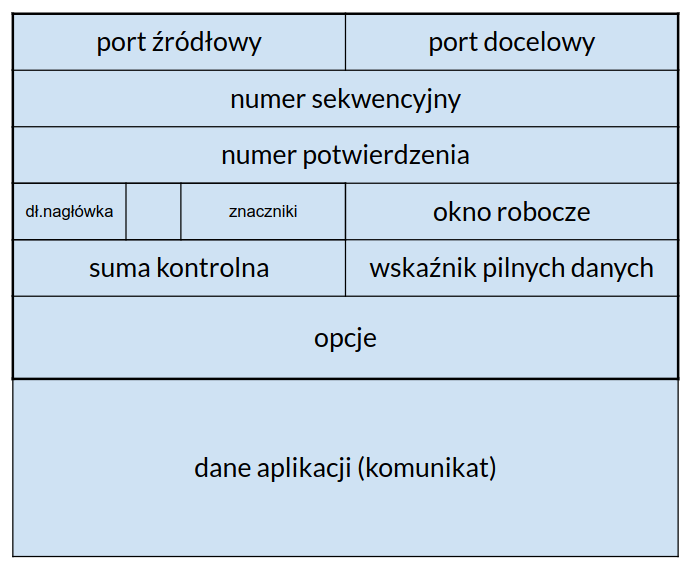
\includegraphics[scale=0.3]{rozdziały/images/SIK/tcp_structure.png}
    \caption{Protokół TCP, struktura segmentu}
\end{figure}

\begin{figure}[H]
    \centering
    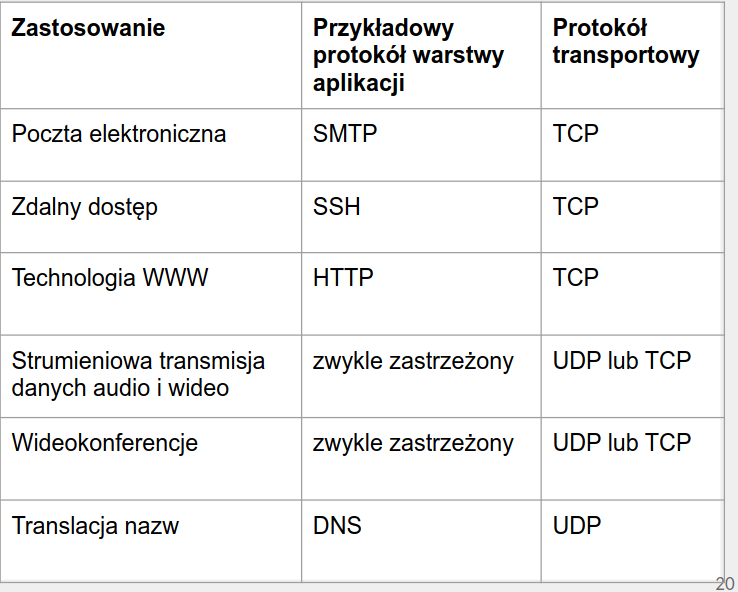
\includegraphics[scale=0.3]{rozdziały/images/SIK/udp_vs_tcp.png}
    \caption{Porównanie zastosowań TCP oraz UDP}
\end{figure}


\subsection{IP}

\begin{figure}[H]
    \centering
    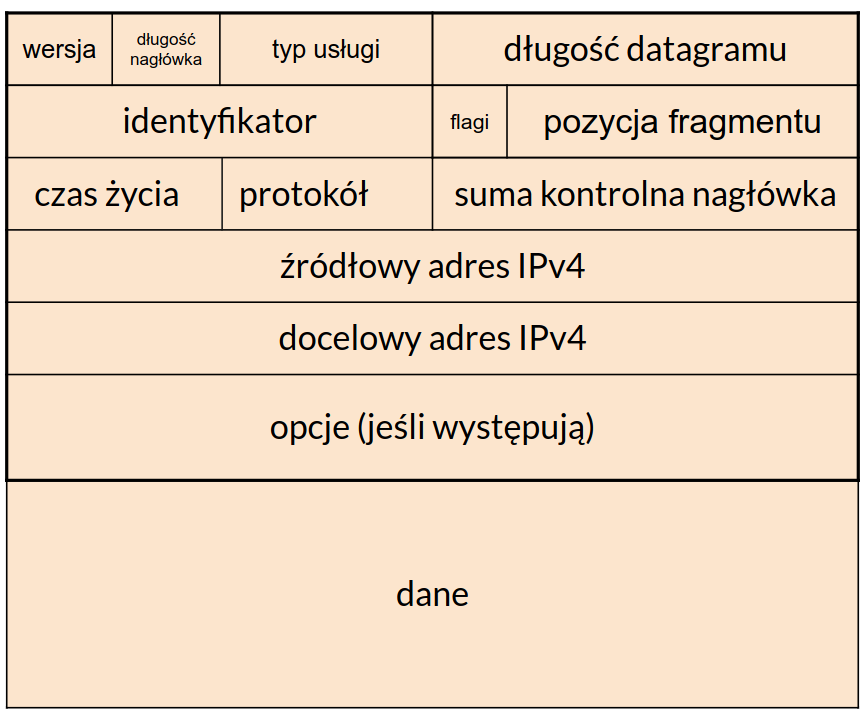
\includegraphics[scale=0.3]{rozdziały/images/SIK/datagram_ipv4.png}
    \caption{Datagram IPv4}
\end{figure}

\begin{itemize}
    \item wersja protokołu IP – 4
    \item długość nagłówka, IHL (Internet Header Length) – liczona w 32-bitowych słowach,
    nagłówek może być maksymalnie 60 bajtowy
    \item typ usługi, ToS (Type of Service) – nieaktualne
    \item całkowita długość datagramu (16 bitów), ograniczenie rozmiaru do $2^{16}$ bajtów
    \item czas życia, TTL (Time To Live) (8 bitów) zmniejszany o 1 przez każdy router
    \item protokół warstwy wyższej (8 bitów), którego pakiet jest przenoszony np. 6 (TCP), 17 (UDP), 41 (IPv6)
    \item źródłowy adres IPv4 (32 bity)
    \item docelowy adres IPv4 (32 bity)
    \item standardowa internetowa suma kontrolna - obliczana tylko dla nagłówka, przetwarzana przez każdy router, zmienna ze względu na zmniejszanie TTL i możliwą zmianę opcji
\end{itemize}

\textbf{Fragmentacja datagramu} \\
Niekiedy konieczny jest podział datagramu na mniejsze pakiety.
\begin{itemize}
    \item nadawca nadaje identyfikator każdemu segmentowi
    \item fragmenty są składane zanim trafią do warstwy transportowej odbiorcy (nie są w routerach)
    \item warstwa sieci odbiorcy posługuje się identyfikatorem, pozycją fragmentu i flagą MF (more fragments) przy defragmentacji datagramu
\end{itemize}


\begin{figure}[H]
    \centering
    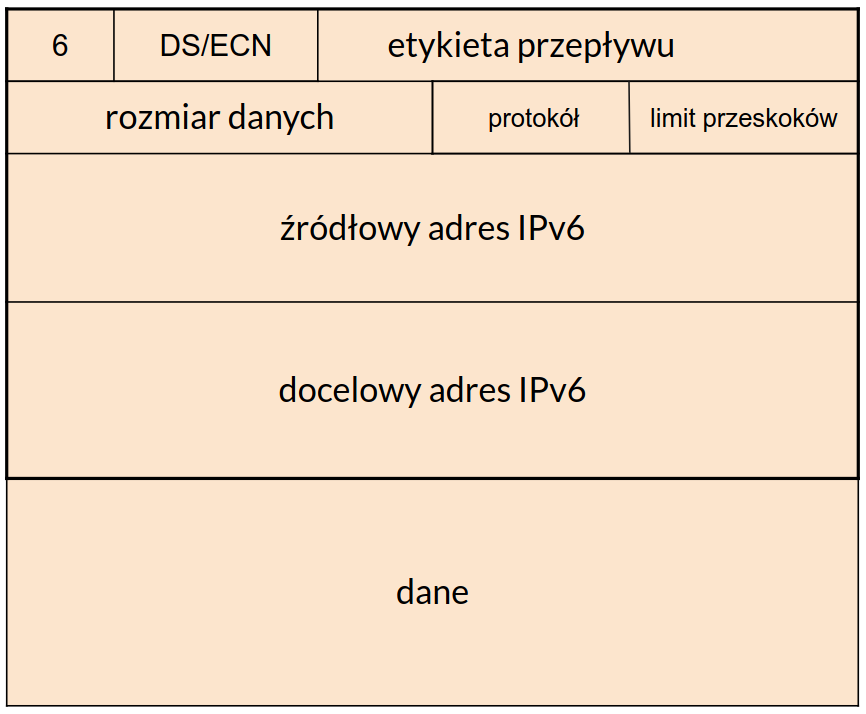
\includegraphics[scale=0.3]{rozdziały/images/SIK/datagram_ipv6.png}
    \caption{Datagram IPv6}
\end{figure}

\begin{itemize}
    \item stały rozmiar nagłówka: 40B
    \item brak sumy kontrolnej 
    \item brak informacji dotyczących fragmentacji ze względu na to, że nie jest ona możliwa na routerach, a jedynie na systemach końcowych, zbyt duży pakiet jest odrzucany przez router
    \item etykieta przepływu – routery mają traktować tak samo datagramy należące do tego samego przepływu
\end{itemize}

\subsection{DHCP}

\textbf{DHCP - Dynamic Host Resolution Protocol}
\begin{itemize}
    \item w każdej sieci, bez względu na rozmiar
    \item przydział ma postać odnawialnej \textbf{dzierżawy}
    \item korzysta z UDP na portach 67 i 68
    \item pierwszy źródłowy adres klienta to 0.0.0.0
    \item docelowy adres serwera DHCP 255.255.255.255, nasłuchuje port 68, wysyła przez 67
    \item klient i serwer identyfikują się za pomocą \textbf{ID transakcji}
\end{itemize}

DHCPv6 ma dwa tryby działania: stanowy (podobny do DHCPv4) i bezstanowy (wykorzystuje autokonfigurację adresów).

Przekaźnik DHCP (agent przekazywania) - rozszerza dostępność DHCP poza sieć lokalną. Zwykle jest to router.

\subsection{ICMP}

Internet Control Message Protocol

\begin{itemize}
    \item uzupełnienie funkcjonalności protokołu IP, 
    \item służy do przesyłania informacji o błędach lub informacji kontrolnych
    \item komunikaty o \textbf{błędach} kierowane są do procesów użytkownika lub do warstwy wyższej (zawierają kopię części datagramu, który był przyczyną błędu)
    \item na ogół komunikatami informacyjnymi zarządza system operacyjny
\end{itemize}

Kiedy komunikaty nie są generowane? 
\begin{itemize}
    \item inne komunikaty ICMP o błędach
    \item datagramy rozgłoszeniowe lub rozsyłania grupowego
    \item datagramy, których adres źródłowy nie określa konkretnego hosta, czyli np. z adresem zerowym, pętli zwrotnej, niepoprawnym
    \item kolejne fragmenty podzielonego datagramu
\end{itemize}

Przykłady komunikatów: 
\begin{itemize}
    \item \textbf{Destination Unreachable},
    \item \textbf{Packet Too Big},
    \item \textbf{Redirect} (jeśli router, zgodnie ze swoją tablicą tras, ma skierować pakiet do tej samej sieci, z której został wysłany, oznacza to błąd trasowania),
    \item \textbf{Time Exceeded} - TTL spadł do 0
    \item \textbf{RS} - zapytanie o router, \textbf{RA} - ogłoszenie routera (przydatne w DHCP)
\end{itemize}

\subsection{Protokoły zapewniające bezpieczeństwo}

\textbf{SSL}

\begin{itemize}
    \item zapewnia bezpieczeństwo protokołu TCP
    \item najczęściej używa się go do ochrony transakcji realizowanych przez protokół HTTP (HTTPS), ale można go zastosować do dowolnej aplikacji korzystającej z TCP
    \item udostępnia oparty na gniazdach interfejs
\end{itemize}

\textbf{IPSec}

\begin{itemize}
    \item zapewnia bezpieczeństwo w warstwie sieci
    \item chroni datagramy IP pomiędzy dwoma węzłami nawiązującymi logiczne połączenie
    \item służy do tworzenia wirtualnych sieci prywatnych, VPN (ang. Virtual Private Network), alternatywy dla sieci prywatnych, gdzie wewnętrzny ruch jest przesyłany w bezpieczny sposób przez sieć publiczną
\end{itemize}


\subsection{Ethernet}


\begin{problems}
    \prob Przechwycono następujące zapytanie HTTP programem Wireshark:
    \begin{verbatim}
        GET /files/docs1.html HTTP/1.1\r\n
        Host: example.com\r\n
        Accept-Encoding: gzip, deflate\r\n
        Accept-Language: pl;q=0.8, en-gb;q=0.2\r\n
        Connection: keep-alive\r\n
        \r\n
    \end{verbatim}
    Wówczas
    \answers{adres URL żądanego zasobu to \text{http://example.com/files/docs1.html}}{ustanawiane jest połączenie nietrwałe}{zadeklarowano obsługę algorytmu kompresji gzip}
    
    \prob IPsec sprawdzi się lepiej niż TCP z SSL do
    \answers{wideo telekonferencji}{przesyłania pliku}{rozmowy telefonicznej}

    \prob W nagłówku TCP znajduje się
    \answers{numer portu nadawcy}{adres IP odbiorcy}{32-bitowy numer kolejny pakietu}

    \prob Protokół DHCP
    \answers{służy do odwzorowania adresów sieciowych IP na adresy sprzętowe MAC}{korzysta z protokołu UDP}{umożliwia wynajęcie adresu IP na określony czas}

    \prob Konflikt w sieci Ethernet
    \answers
    {występuje w wyniku błędnej konfiguracji}
    {jest naturalnym zjawiskiem rozwiązywanym przez mechanizm CSMA/CD}
    {występuje gdy występują dwa urządzenia o tym samym adresie MAC}

    \prob W sieciach TCP/IP zbudowanych w oparciu o technologię Ethernet parametr MTU oznacza
    \answers
    {maksymalny rozmiar pola danych ramki Ethernetowej}
    {maksymalny rozmiar segmentu danych TCP}
    {maksymalny rozmiar datagramu IP, który nie wymaga jeszcze stosowania fragmentacji}
  

    \prob Nagłówek datagramu IP zawiera między innymi
    \answers
    {numer wersji tego protokołu}
    {adres IP nadawcy}
    {numer portu nadawcy}

    \prob Protokół ARP służy do
    \answers
    {wiązania adresu fizycznego komputera z adresem IP}
    {wiązania nazwy komputera z adresem IP}
    {wiązania nazwy komputera z adresem fizycznym}

    \prob Host $A$ przesyła przez TCP plik o rozmiarze 1GiB do hosta $B$. $B$ w warstwie aplikacji nie wysyła nic do $A$. Wynika stąd, że
    \answers{host $A$ wyśle więcej niż 2020 segmentów z flagą ACK do $B$}{host $A$ czeka na potwierdzenie każdego segmentu przed wysłaniem kolejnego}{liczba niepotwierdzonych bajtów wysłanych przez $A$ nigdy nie jest większa niż rozmiar okna roboczego $B$}
\end{problems}

% Kasia
\section{Adresy internetowe, tablice tras, zasady trasowania, NAT}

\subsection{Adresy IP}

Adresy IPv4 32-bitowe:
\begin{center}
    \begin{tabular}{|c|c|}
        \hline
        Reprezentacja dziesiętna & Reprezentacja binarna \\
        \hline
         10.1.0.122 & 00001010 00000001 00000000 01111010 \\
         193.0.96.129 & 11000001 00000000 01100000 10000001 \\
         \hline
    \end{tabular} \\
\end{center}

Adresy IPv6 128-bitowe:
\begin{center}
    \begin{tabular}{|c|c|}
        \hline
        Reprezentacja szesnastkowa & Reprezentacja uproszczona \\
        \hline
        2001:06a0:5001:0002:34ed:69ae:55aa:7f61  & 2001:6a0:5001:2:34ed:69ae:55aa:7f61 \\
         2001:db8:0:0:0:0:0:2  & 2001:db8::2 \\
         \hline
    \end{tabular}
\end{center}

Zasady upraszczania reprezentacji szesnastkowej:
\begin{itemize}
    \item cyfry małymi literami, usuwanie wiodących zer
    \item redukcja najdłuższego spójnego ciągu zer
\end{itemize}

IPv6 bywa zapisywane w kwadratowych nawiasach np. http://[2001:db8:85a3:8d3:1319:8a2e:370:7348]

\textbf{Historyczne klasy adresów IPv4}

\begin{figure}[H]
    \centering
    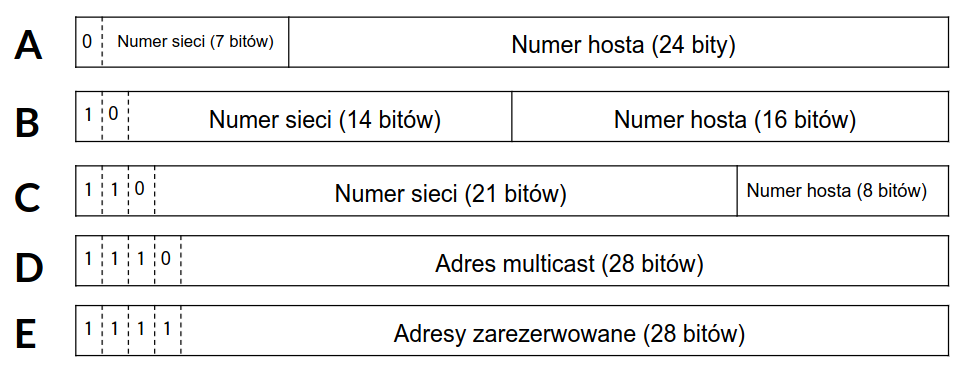
\includegraphics[scale=0.4]{rozdziały/images/SIK/klasy_ipv4.png}
\end{figure}

\textbf{CIDR - Classless Inter-Domain Routing}
\begin{itemize}
    \item zapewnia adresowanie bezklasowe
    \item wymaga wprowadzenia maski CIDR (prefiksu) 
\end{itemize}

\begin{center}
    \centering
    \begin{tabular}{|c|c|c|}
         \hline
         Reprezentacja bitowa & Zapis dziesiętny & Zapis prefiksowy \\
         \hline
         10000000 00000000 00000000 00000000 & 128.0.0.0 & /1 \\
         11111111 11000000 00000000 00000000 & 255.192.0.0 & /10 \\
         \hline
    \end{tabular}
\end{center}

Nakładanie maski - koniunkcja bitowa.

\begin{center}
    \centering
    \begin{tabular}{|c|c|c|}
         \hline
         Adres & 00001010 00000010 00000110 10110011 & 10.2.6.179 \\
         \hline
         Maska podsieci & 11111111 11111111 11111111 00000000 & 255.255.255.0 \\
         \hline
         Adres sieci & 00001010 00000010 00000110 00000000 & 10.2.6.0/24 \\
         \hline
    \end{tabular}
\end{center}

Obliczanie liczby urządzeń w sieci: $2^{32 - \text{\# bitów maski}} - 2$.

\textbf{Adresy specjalne}

\textbf{Adres rozgłoszeniowy} - alternatywa bitowa z zanegowaną maską. Jest to największy adres w sieci. 
\begin{center}
    \centering
    \begin{tabular}{|c|c|c|}
         \hline
         Adres & 00001010 00000010 00000110 10110011 & 10.2.6.179 \\
         \hline
         Zanegowana maska & 00000000 00000000 00000000 11111111 & 0.0.0.255 \\
         \hline
         Wynik & 00001010 00000010 00000110 11111111 & 10.2.6.255 \\
         \hline
    \end{tabular}
\end{center}

\begin{itemize}
    \item 255.255.255.255/32 - ostatni adres z przestrzeni adresowej IPv4 - ograniczone rozgłaszanie lokalne, 
    \item 127.0.0.0/8 - wszystkie adresy z tej sieci są adresami loopback, czyli wskazuje na bieżący węzeł; taki adres może być tylko \textbf{docelowym} adresem paczki,
    \item 224.0.0.0/4 - rozgłaszanie grupowe - od 224.0.0.0 do 239.255.255.255,
    \item 0.0.0.0/8 - wyłącznie adres źródłowy (np. kiedy nie jest jeszcze znany)
\end{itemize}

\textbf{Adresy prywatne} - mogą być używane tylko w sieci lokalnej - nie są rutowalne w sieci publicznej. \quad \textbf{\red{(przyp. red.: jakie to są adresy prywatne? dobrze byłoby to wyjaśnić)}}

\begin{center}
    \centering
    \begin{tabular}{|c|c|c|c|}
         \hline
         Prefiks & Pierwszy adres & Ostatni adres & Rozmiar \\
         \hline
         10.0.0.0/8 & 10.0.0.1 & 10.255.255.254 & $2^{24}-2$\\
         \hline
         172.16.0.0/12 & 172.16.0.1 & 172.31.255.254 & $2^{20}-2$ \\
         \hline
         192.168.0.0/16 & 192.168.0.1 & 192.168.255.254 & $2^{16}-2$\\
         \hline
    \end{tabular}
\end{center}

\begin{example}
    Rozważmy sieć o masce /15. W tej sieci znajduje się komputer o adresie \textbf{111.96.99.74}. \\
    Podaj liczbę dostępnych adresów dla urządzeń w tej sieci. -- $2^{17} - 2$.\\
    Czy adres 111.97.187.73 należy do tej sieci? -- Tak, bo obydwa adresy należą do sieci 111.96.0.0
\end{example}

\subsection{Przydzielanie adresów IP}

Rodzaje: 
\begin{itemize}
    \item ręczne
    \item dynamiczne, za pomocą usług sieciowych
    \item automatyczne
\end{itemize}

\subsection{Trasowanie}

Algorytmy trasowania:   
\begin{itemize}
    \item algorytm stanu łącza
    \item algorytm wektora odległości
\end{itemize}

\begin{figure}[H]
    \centering
    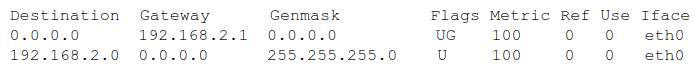
\includegraphics[scale=0.5]{rozdziały/images/SIK/tablica_tras.png}
\end{figure}

Elementy tablicy tras:
\begin{itemize}
    \item \textbf{przeznaczenie} – razem z polem maski stanowi kryteria dopasowania adresu
    docelowego, wartość zerowa odpowiada trasie domyślne
    \item \textbf{brama} - adres następnego węzła, wartość zerowa oznacza sieć lokalną
    \item \textbf{maska} - zostaje nałożona na adres docelowy, po czym następuje próba dopasowania wyniku do któregoś z pól przeznaczenia
    \item flagi, koszt, liczniki odwołań
    \item interfejs, który powinien dostarczyć datagram
\end{itemize}

\begin{example}
    Tablica tras dla routera R2.

    \begin{figure}[H]
    \centering
    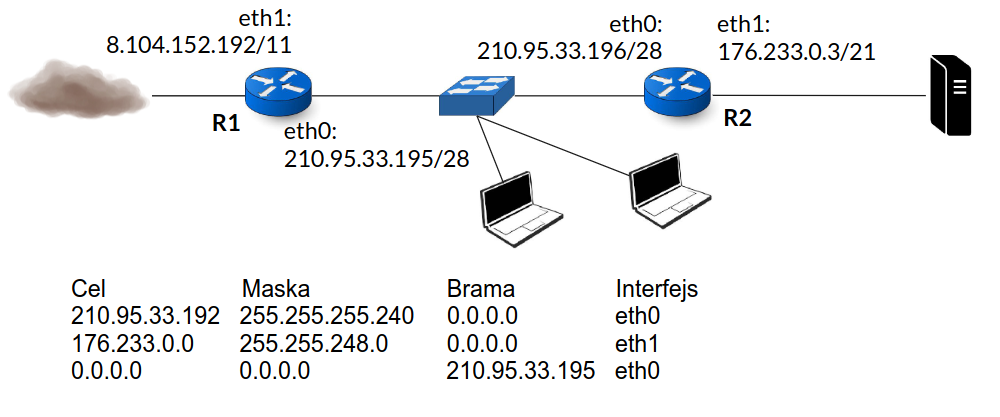
\includegraphics[scale=0.4]{rozdziały/images/SIK/nat_przyklad.png}
\end{figure}
\end{example}

Zasady dopasowania w trasowaniu:
\begin{itemize}
    \item adres docelowy datagramu pasuje do trasy, jeśli jego koniunkcja bitowa z maską dla tej trasy daje w wyniku wartość pola przeznaczenie
    \item w przypadku wielu pasujących tras wybierany jest trasa z najdłuższym pasującym prefiksem (czyli z najdłuższą maską)
    \item jeśli nie zostanie odnaleziona pasująca trasa, to aplikacja dostanie komunikat “Network unreachable” lub do nadawcy zostanie wysłany odpowiedni komunikat ICMP
\end{itemize}

\begin{example}
    \begin{figure}[H]
    \centering
    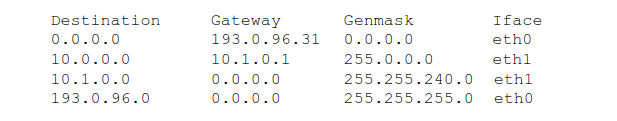
\includegraphics[scale=0.5]{rozdziały/images/SIK/trasowanie_przyklad.png}
    
    Nałożenie maski 255.255.255.0 na adres \textbf{193.0.96.42} daje w wyniku 193.0.96.0, więc adres pasuje do trasy czwartej. \\
    Adres \textbf{10.1.0.42} pasuje do pozycji pierwszej, drugiej i trzeciej, wybrana zostanie trzecia.
\end{figure}
\end{example}

\subsection{NAT}
Network Address Translation 
\begin{itemize}
    \item adres źródłowy, który jest adresem prywatnym zostaje zamieniony na adres globalny jakim dysponuje router NAT
    \item router z funkcją NAT oddziela prywatną sieć od internetu
    \item translacja odpowiedzi odbywa się w przeciwną stronę – globalny adres zostaje zamieniony na oryginalny adres prywatny
\end{itemize}

\begin{problems}
    \prob Jeśli ruter musi przesłać datagram IP w wersji 4 o całkowitej długości 4500 oktetów w sieci o MTU 1500, to
    \answers{podzieli go na 3 fragmenty}{zawsze w nagłówku drugiego fragmentu ustawi znacznik, że są jeszcze dalsze fragmenty}{zawsze w nagłówku ostatniego fragmentu ustawi znacznik zabraniający dalszej fragmentacji}

    \prob Ruter o co najmniej dwóch interfejsach sieciowych ma między innymi adresy fizyczne 202.107.123.15/26, 150.192.0.20/19. Brama domyślna w jego tablicy tras ma najmniejszy możliwy adres w swojej sieci. Możliwe adresy bramy domyślnej to:
    \answers{202.107.123.1}{150.192.0.1}{inny niż 202.107.123.1 i 150.192.0.1}
    
    \prob Mamy do dyspozycji sieć IPv4 klasy C. Chcemy podzielić ją na co najmniej 4 podsieci po co najmniej 16 urządzeń w każdej. Pozwoli nam na to maska
    \answers{255.255.255.192}{255.255.255.224}{255.255.255.240}

    \prob W sieci fizycznej, w której znajduje się maszyna o adresie $77.145.123.18/20$,
    \answers{adresem IP urządzenia może być $77.145.112.255$}{adresem ukierunkowanego rozgłaszania jest $77.145.123.255$}{można zaadresować $2^{20} - 2 = 1048574$ urządzenia}

    \prob Adres planowanej sieci należy do dawnej klasy C. Chcemy podzielić sieć na co najmniej $5$ podsieci, tak aby w każdej znalazło się co najmniej $16$ urządzeń. Realizację tego wymagania zapewnia maska
    \answers{$255.255.255.240$}{$255.255.255.224$}{$255.255.255.192$}

    \prob W sieci publicznej nierutowalnymi adresami są:
    \answers
    {127.0.0.1}
    {10.1.1.2}
    {174.49.2.87}

\end{problems}

\section{Systemy nazw domenowych}

\textbf{DNS} - Domain Name System - zapewnia odwzorowanie nazwy na adres IP. Korzysta z protokołu DNS (port 53).

Serwery w hierarchii DNS:
\begin{itemize}
    \item serwery główne
    \item TLD - serwery domen najwyższego poziomu (com, edu, net)
    \item serwery autorytatywne - każda organizacja dysponująca serwerami publicznie dostępnymi musi udostępniać odwzorowanie ich nazw na adresy IP
\end{itemize}

\textbf{Serwery lokalne} - pierwszy krok w rozwiązywaniu nazwy. Obsługują zapytania klientów. Nie należą do hierarchii DNS.

\textbf{Pliki strefy} zawierają rekordy, czyli (nazwa, klasa, typ, wartość). Do typów należą m.in. (A - IPv4 hosta, AAAA-  IPv6 hosta, MX - nazwa kanoniczna serwera pocztowego).


\begin{problems}
     \prob W usłudze DNS
    \answers{każde zapytanie kierowane jest do głównego serwera IANA}{możliwe jest poznanie nazwy komputera z jego adresu IP}{wymagane jest użycie klienta Ethernetu jako drugiej warstwy sieciowej}
    
\end{problems}

\section{Sieciowy interfejs gniazd}

\textbf{Gniazda BSD} (BSD sockets): interfejs pomiędzy programami użytkowników a implementacją stosu TCP/IP. Procesy komunikują się za pomocą modelu klienta i serwera.

Tryby komunikacji gniazd: bezpołączeniowy (UDP) i połączeniowy (TCP).

Klient musi mieć informacje o adresie, porcie i protokole na którym serwer nasłuchuje. Serwer nie musi mieć informacji o kliencie – dostaje informacje po nawiązaniu komunikacji.

\begin{solutions}
    % Kasia K
    \sol Przechwycono następujące zapytanie HTTP programem Wireshark:
    \begin{verbatim}
        GET /files/docs1.html HTTP/1.1\r\n
        Host: example.com\r\n
        Accept-Encoding: gzip, deflate\r\n
        Accept-Language: pl;q=0.8, en-gb;q=0.2\r\n
        Connection: keep-alive\r\n
        \r\n
    \end{verbatim}
    Wówczas
    \answerss{adres URL żądanego zasobu to \texttt{http://example.com/files/docs1.html}}{ustanawiane jest połączenie nietrwałe}{zadeklarowano obsługę algorytmu kompresji gzip}{TAK}{NIE}{TAK}

    \begin{enumerate} [\bf A.]
        \item Łączymy informacje o protokole (\texttt{http}), hoście (\texttt{example.com}) oraz ścieżki zapytania (\texttt{/files/docs1.html}) zgodnie z zasadami tworzenia zapytań HTTP otrzymując adres z pytania.
        \item  Zdefiniowane w zapytaniu \texttt{Connection: keep-alive} oznacza, że połączenie jest trwałe.
        \item  Zdefiniowane w zapytaniu \texttt{Accept-Encoding: gzip} oznacza umiejętność obsługi kompresji gzip.
    \end{enumerate}

    % Grześ
    \sol IPsec sprawdzi się lepiej niż TCP z SSL do
    \answerss{wideo telekonferencji}{przesyłania pliku}{rozmowy telefonicznej}{TAK}{NIE}{TAK}
    IPsec korzysta z UDP, które nie nadaje się do przesyłania plików, ponieważ raczej chcemy, żeby plik dotarł do odbiorcy w całości. Jeśli chodzi o wideo telekonferencje i rozmowy telefoniczne, to najważniejsze, by rozmowa była płynna, w czym lepiej poradzi sobie protokół UDP.

    % Kasia K
    \sol W nagłówku TCP znajduje się
    \answerss{numer portu nadawcy}{adres IP odbiorcy}{32-bitowy numer kolejny pakietu}{TAK}{NIE}{TAK}
    \begin{enumerate} [\bf A.]
        \item Wprost z grafiki ze strukturą.
        \item To dopiero jest w warstwie sieci.
        \item Wprost z grafiki ze strukturą.
    \end{enumerate}

    % Grześ
    \sol Protokół DHCP
    \answerss{służy do odwzorowania adresów sieciowych IP na adresy sprzętowe MAC}{korzysta z protokołu UDP}{umożliwia wynajęcie adresu IP na określony czas}{NIE}{TAK}{TAK}
    \textbf{A.} To nie jest ARP, tylko DHCP.

    \textbf{B.} Owszem, na portach 67 i 68.

    \textbf{C.} No tak.

    \sol Konflikt w sieci Ethernet
    \answerss
    {występuje w wyniku błędnej konfiguracji}
    {jest naturalnym zjawiskiem rozwiązywanym przez mechanizm CSMA/CD}
    {występuje gdy występują dwa urządzenia o tym samym adresie MAC}
    {NIE}{TAK}{NIE}
    (sprawdzić, czy da się uzupełnić to zadanie, tak żeby miało dydaktyczny sens)

    % Grześ
    \sol W sieciach TCP/IP zbudowanych w oparciu o technologię Ethernet parametr MTU oznacza
    \answerss
    {maksymalny rozmiar pola danych ramki Ethernetowej}
    {maksymalny rozmiar segmentu danych TCP}
    {maksymalny rozmiar datagramu IP, który nie wymaga jeszcze stosowania fragmentacji}
    {NIE}{NIE}{TAK}
    Wystarczy przeczytać, czym jest MTU i odpowiedzi stają się jasne.

    \sol Nagłówek datagramu IP zawiera między innymi
    \answerss
    {numer wersji tego protokołu}
    {adres IP nadawcy}
    {numer portu nadawcy}
    {TAK}{TAK}{NIE}
    \textbf{A.} Wprost z grafiki o datagramie IP.
    
    \textbf{B.} Źródłowy adres IP jest elementem nagłówka -- wprost z grafiki o datagramie IP.
    
    \textbf{C.} To jest w nagłówku warstwy transportowej.

    % Grześ
    \sol Protokół ARP służy do
    \answerss
    {wiązania adresu fizycznego komputera z adresem IP}
    {wiązania nazwy komputera z adresem IP}
    {wiązania nazwy komputera z adresem fizycznym}
    {TAK}{NIE}{NIE}
    Protokół ARP służy do tłumaczenia adresu sieciowego IP na adres sprzętowy MAC, czyli dokładnie podpunkt \textbf{A.}

    \sol Host $A$ przesyła przez TCP plik o rozmiarze 1GiB do hosta $B$. $B$ w warstwie aplikacji nie wysyła nic do $A$. Wynika stąd, że
    \answerss{host $A$ wyśle więcej niż 2020 segmentów z flagą ACK do $B$}{host $A$ czeka na potwierdzenie każdego segmentu przed wysłaniem kolejnego}{liczba niepotwierdzonych bajtów wysłanych przez $A$ nigdy nie jest większa niż rozmiar okna roboczego $B$}{NIE}{NIE}{TAK}
    \textbf{A.} Host $A$ nie musi wcale wysłać tylu segmentów z flagą $ACK$, bo $B$ nie wysyła nic do $A$. Na początku połączenia podadzą sobie rękę, ale to nie będzie $2020$ segmentów.
    
    \textbf{B.} Nie jest tak, wykorzystywane jest buforowanie.
    
    \textbf{C.} Tak działa okno robocze $B$, nie możemy umieścić w buforze więcej bajtów, niż jest w nim w ogóle dostępne.

    \sol Jeśli ruter musi przesłać datagram IP w wersji 4 o całkowitej długości 4500 oktetów w sieci o MTU 1500, to
    \answerss{podzieli go na 3 fragmenty}{zawsze w nagłówku drugiego fragmentu ustawi znacznik, że są jeszcze dalsze fragmenty}{zawsze w nagłówku ostatniego fragmentu ustawi znacznik zabraniający dalszej fragmentacji}{NIE}{TAK}{NIE}
    Datagram IP zawiera nagłówek oraz resztę danych. Dzieląc go na fragmenty za każdym razem powielamy nagłówek, a dane jakoś dzielimy. Stąd w \textbf{A.} podzielimy go na więcej niż 3 fragmenty. \textbf{B.} tak jest po prostu, logiczne. \textbf{C.} skoro jest to co w \textbf{B.}, to to by już było useless, nie ma tego.

    \sol Ruter o co najmniej dwóch interfejsach sieciowych ma między innymi adresy fizyczne 202.107.123.15/26, 150.192.0.20/19. Brama domyślna w jego tablicy tras ma najmniejszy możliwy adres w swojej sieci. Możliwe adresy bramy domyślnej to:
    \answerss{202.107.123.1}{150.192.0.1}{inny niż 202.107.123.1 i 150.192.0.1}{TAK}{TAK}{TAK}

    Adres 202.107.123.15 ma maskę 26, czyli zmienić możemy jedynie ostatnie 6 bitów w adresie. W adresie 150.192.0.20 z maską 19 możemy zmienić 5 młodszych bitów w 3-cim od lewej bajcie i wszystkie 8 w najbardziej prawym. \textbf{A.} adres 202.107.123.1 jest adresem urządzenia w pierwszej sieci, więc ok. \textbf{B.} tak samo, ustawiamy wszystkie bity oprócz ostatniego na 0 i jest ok. \textbf{C.} wiemy, ze ruter ma co najmniej dwa interfejsy i podane są dwa przykłady adresów, ale może być ich więcej -- nie wiemy tego.

    % Patryk
    \sol Mamy do dyspozycji sieć IPv4 klasy C. Chcemy podzielić ją na co najmniej 4 podsieci po co najmniej 16 urządzeń w każdej. Pozwoli nam na to maska
    \answerss{255.255.255.192}{255.255.255.224}{255.255.255.240}{TAK}{TAK}{NIE}
    (\textbf{A.} dla bardzo starych sieci (sprzed roku 1995) to może nie działać. Patrz: \url{https://www.cisco.com/c/en/us/support/docs/ip/dynamic-address-allocation-resolution/13711-40.html#problemswithsubnetzero}. W oryginalnej wersji zadania było wspomniane, że sieć jest stara (i dlatego mamy do czynienia z klasami), ale nie było powiedziane, jak bardzo stara, więc obie odpowiedzi się bronią.)

    \textbf{\red{Przyp. red.: dopisać rozwiązanie do tego zadania (obecnie brak wyjaśnienia, dlaczego odpowiedzi są takie, a nie inne) oraz przerzucić całe to zadanie do ramki ,,To było na egzaminie'' w sensownym miejscu w części teoretycznej -- istnieje już bardzo analogiczne zadanie, więc nie ma sensu, żeby się dublowało w tym zestawie zadań.}}

    \sol W sieci fizycznej, w której znajduje się maszyna o adresie $77.145.123.18/20$,
    \answerss{adresem IP urządzenia może być $77.145.112.255$}{adresem ukierunkowanego rozgłaszania jest $77.145.123.255$}{można zaadresować $2^{20} - 2 = 1048574$ urządzenia}{TAK}{NIE}{NIE}
    Mamy maskę 20, więc 20 najbardziej lewych bitów jest ustawione. Adres sieci to zatem 77.145.112.0, a adres rozgłoszeniowy to 77.145.127.255. \textbf{A.} 77.145.112.255 jest pomiędzy adresem sieci a rozgłoszeniowym -- git. \textbf{B.} Nie. \textbf{C.} Z maską równą $k$ można w $IPv4$ adresować $2^{32-k}-2$ urządzeń, czyli tutaj $2^{12}-2=4094$.

    % Patryk
    \sol Adres planowanej sieci należy do dawnej klasy C. Chcemy podzielić sieć na co najmniej $5$ podsieci, tak aby w każdej znalazło się co najmniej $16$ urządzeń. Realizację tego wymagania zapewnia maska
    \answerss{$255.255.255.240$}{$255.255.255.224$}{$255.255.255.192$}{NIE}{TAK}{NIE}

    \sol W sieci publicznej nierutowalnymi adresami są:
    \answerss
    {127.0.0.1}
    {10.1.1.2}
    {174.49.2.87}
    {TAK}{TAK}{NIE}

    \sol W usłudze DNS
    \answerss{każde zapytanie kierowane jest do głównego serwera IANA}{możliwe jest poznanie nazwy komputera z jego adresu IP}{wymagane jest użycie klienta Ethernetu jako drugiej warstwy sieciowej}{NIE?}{TAK?}{NIE?}
    (być może w \textbf{B.} chodzi o reverse DNS)
\end{solutions}